\documentclass[11pt, a4paper]{article}

\usepackage{graphicx}
\usepackage[a4paper,top=3cm,bottom=2cm,left=2cm,right=2cm,marginparwidth=1.75cm]{geometry}
\usepackage[english]{babel}
\usepackage[utf8x]{inputenc}
\usepackage{subfig}
\usepackage{float}
\usepackage{amsmath}
\usepackage{amssymb}
\usepackage{mhchem}
\usepackage{hyperref}
\usepackage{tikz}
\usepackage{cancel}

\graphicspath{ {./images} }
\newcommand*{\qed}{\hfill\ensuremath{\quad\square}}%
\newcommand*{\rad}{\ensuremath{\,\text{rad}}}
\newcommand*{\R}{\ensuremath{\mathbb{R}}}
\newcommand*{\C}{\ensuremath{\mathbb{C}}}
\renewcommand*{\Re}{\operatorname{Re}}
\renewcommand*{\Im}{\operatorname{Im}}
\renewcommand*{\epsilon}{\varepsilon}
\renewcommand*{\phi}{\varphi}

\makeatletter
\renewcommand*\env@matrix[1][*\c@MaxMatrixCols c]{%
  \hskip -\arraycolsep
  \let\@ifnextchar\new@ifnextchar
  \array{#1}}
\makeatother

\newtheorem{theorem}{Theorem}

%------------------------------------------------
%Templates for images and figures
% \begin{figure}[h]
%   \centering
%   \subfloat[caption 1]{{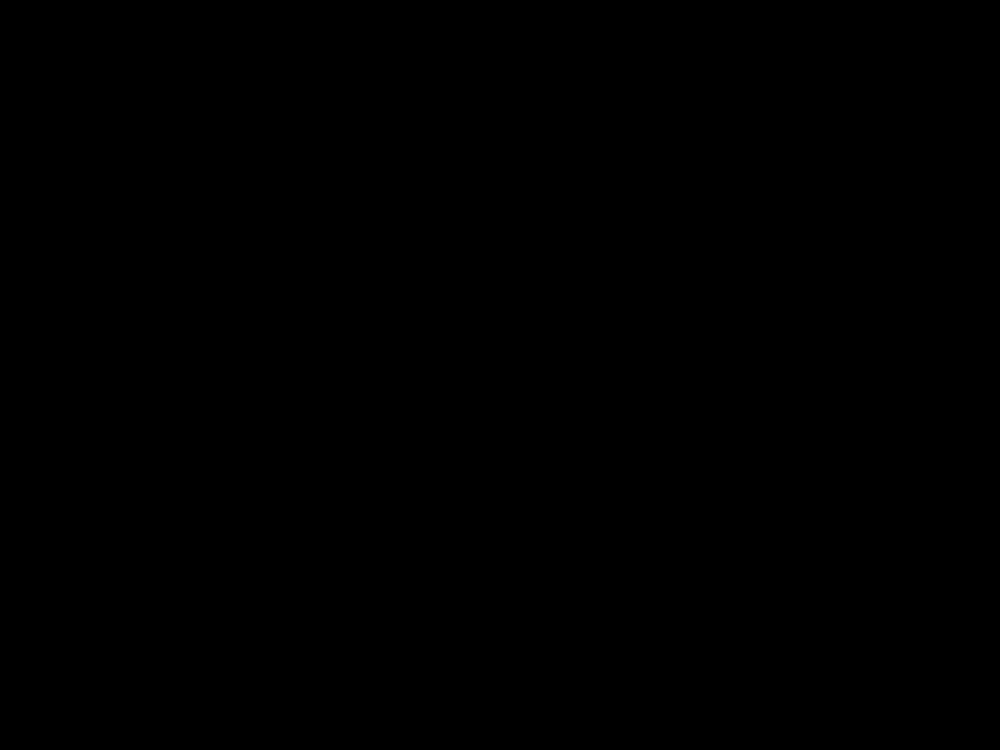
\includegraphics[width=30mm]{images/placeholder.png}}}%
%   \qquad
%   \subfloat[caption 2]{{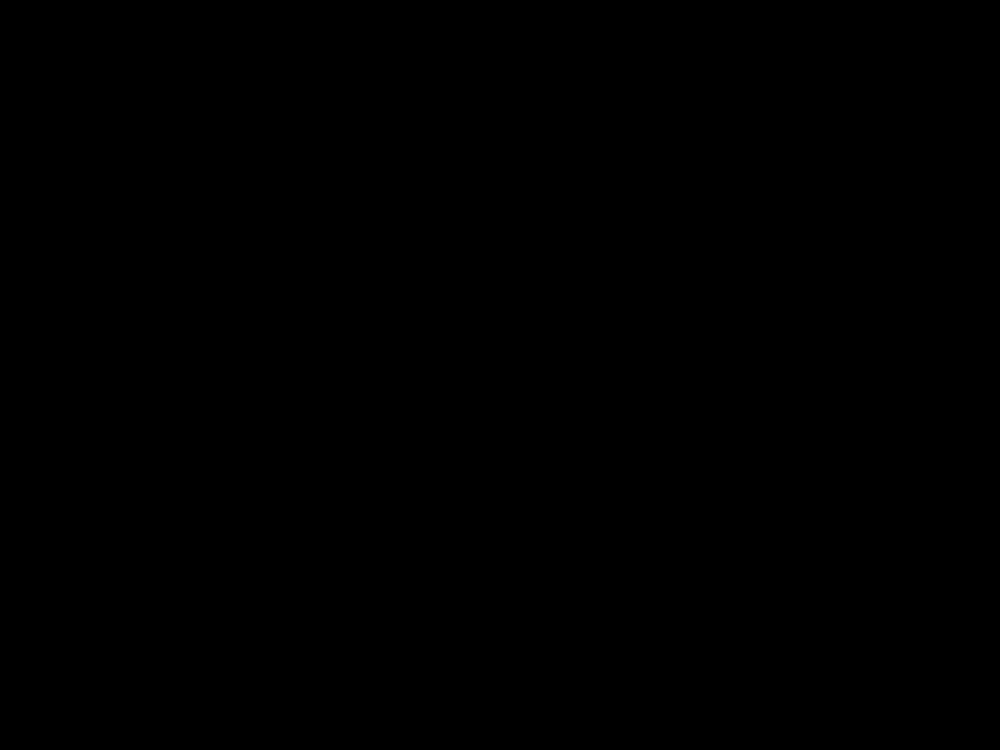
\includegraphics[width=30mm]{images/placeholder.png}}}%
%   \caption{Description}
% \end{figure}

% \begin{figure}[h]
%   \centerline{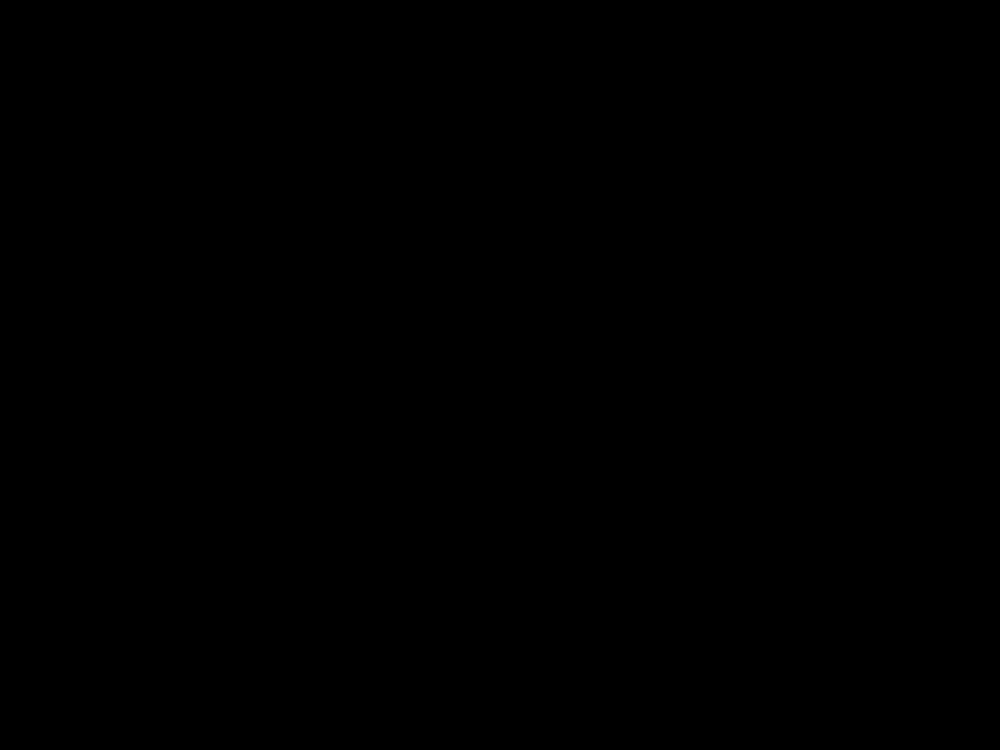
\includegraphics[width=50mm]{images/placeholder.png}}
%   \caption{Description}
% \end{figure}

%Template for a simple table 
%\begin{table}[h]
%   \caption{Description} %title of the table
%   \centering % centering table
%   \begin{tabular}{l rr} % creating three columns
%     \hline\hline %inserting double-line
%     & & \\ [0.5ex] % Insert half line vertical spacing
%     \hline % inserts single-line
%     & & \\ 
%     & & \\
%     & & \\
%     & & \\
%   \hline % inserts single-line
%   \end{tabular}
%   \label{tab:hresult}
% \end{table}
%-----------------------------------------------

\begin{document}
\setcounter{section}{10}
\setcounter{equation}{0}

\section{Linear Algebra Lecture 11: Constrained optimization (02/06/2020)}


\subsection{Constraining functions}
For any objective function $f(\vec{x})$ constraints need to be defined in order to optimize it. Finding the max value of a function $f(\vec{x}) = x_1^2 + x_2^2$ doesn't really make sense when considering all possible values. When we take one of the bounds at $-\infty$ and $+\infty$ the function also blows up to infinity. This doesn't give us any information other then $f(\vec{x})$ get arbitrarily large for some random large value of $x_1$ or $x_2$. Thus we need to define constraints limiting the area we consider to find the maximal and minimal values. In the table below some functions with examples of possible constraints are listed.
\begin{table}[h]
  \caption{Some examples of objective functions and the constraints that can be placed on them} %title of the table
  \centering % centering table
  \begin{tabular}{l|r} % creating three columns
    \hline\hline %inserting double-line
    Objective function &  Constraints\\ [0.5ex] % Insert half line vertical spacing
    \hline \hline% inserts single-line
    $f(\vec{x}) = x_1 + 2x_2 - 10x_3$ & $x_i \geq 0$ for all $i$\\ 
    $f(\vec{x}) = \exp(x_1)\cos(\pi x_2)$ & $||\vec{x}|| = x_1^2 + x_2^2 = 1$ \\
    $f(\vec{x}) = \exp(x_1)\cos(\pi x_2)$ & $A\vec{x} = \vec{b}$ \\
  \hline % inserts single-line
  \end{tabular}
  \label{tab:hresult}
\end{table}
Note that more exotic functions like $\exp(x_1)\cos(\pi x_2)$ can be approximated as a polynomial using a Taylor series. This makes this technique of optimization both very powerfull and very widely applied in physics and engineering.\\
\\
An example problem: Optimize $Q(\vec{x}) = 3x_1^2 + 7x_2^2$ with the constraint $||\vec{x}|| \leq 1$. A visualisation of this problem is given in figure \ref{fig:optProb}
\begin{figure}[h]
  \centerline{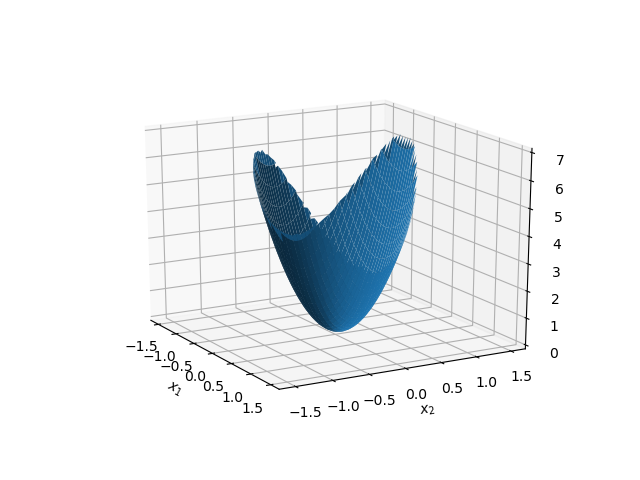
\includegraphics[width=100mm]{images/Figure_1.png}}
  \caption{The visualisation of the function $Q(x_1, x_2)$ and the constraint placed on it}
  \label{fig:optProb}
\end{figure}
To find the maximum and minimum values of this quadratic form we recognize that both terms are positive. Thus:
\begin{align*}
  3x_1^2 + 7x_2^2 &\leq 7x_1^2 + 7x_2^2\\
  &= 7(x_1^2 + x_2^2)\\
  &= 7
\end{align*}
Thus the maximum value is $7$ and occurs at the following points:
\begin{equation*}
  \vec{x} = \pm 
  \begin{bmatrix}
    0\\
    1\\
  \end{bmatrix}
\end{equation*}
This same reasoning also applies to the minimu values:
\begin{align*}
  3x_1^2 + 7x_2^2 &\geq 3x_1^2 + 3x_2^2\\
  &= 3(x_1^2 + x_2^2)\\
  &= 3
\end{align*}
Thus the minimum occurs at the following vectors:
\begin{equation*}
  \vec{x} = \pm 
  \begin{bmatrix}
    1\\
    0\\
  \end{bmatrix}
\end{equation*}


\subsection{Maximal and minimal values}
Let $A$ be an $n \times n$ symmetric matrix with the eigenvalues $\lambda_1 \geq \lambda_2 \geq \cdots \geq \lambda_n$. Then:
\begin{itemize}
  \item The maximal value of $\vec{x}^T A \vec{x}$ under the constraint $||\vec{x}|| = 1$ is $\lambda_1$. This value is attained if $\vec{x}$ is any unit eigenvector of $A$ corresponding to $\lambda_1$.
  \item The minimal value of $\vec{x}^T A \vec{x}$ under the constraint $||\vec{x}|| = 1$ is $\lambda_1$. This value is attained if $\vec{x}$ is any unit eigenvector of $A$ corresponding to $\lambda_n$.
\end{itemize}


\subsection{Quadratic Optimization}
Let $A$ be an $n \times n$ symmetric matrix with eigenvalues $\lambda_1 \geq \cdots \geq \lambda_n$ and the corresponding orthonormal set of eigenvectors $\{\vec{u}_1, \cdots, \vec{u}_n \}$. The the maximal value of $\vec{x}^T A \vec{x}$ subject to he following constraints: $||\vec{x}|| = 1, \vec{x}\cdot \vec{u}_1 = 0, \cdots, \vec{x}\cdot \vec{u}_{k-1} = 0$ is equal to the eigenvalue $\lambda_k$ and this maximla value is attained at $\vec{x} = \pm\vec{u}_k$


\subsection{Example problem}
What is the maximal value of $9x_1^2 + 4x_2^2 + 3x_3^2$ subject to the following constraint: $||\vec{x}|| = 1, \vec{x}\cdots \vec{u} = 0$, where $\vec{u} = \left[1\quad 0\quad 0 \right]^T$. If $\vec{x}\cdot \vec{u}=0$, then: $x_1 = 0$:
\begin{align}
  9x_1^2 + 4x_2^2 + 3x_3^2 &= 4x_2^2 + 3x_3^2\\
  &\leq 4x_2^2 + 4x_3^2\\
  &\leq 4
\end{align}
Thus the maximal value is $4$ and is attained in:
\begin{equation*}
  \vec{x} = \pm
  \begin{bmatrix}
    0\\
    1\\
    0
  \end{bmatrix}
\end{equation*}

\end{document}